\documentclass[12pt]{article}

\input{hw-preamble}
\usepackage{caption}
\usepackage{subcaption}
\usepackage{tikz}
\usepackage{svg}

\begin{document}
\thispagestyle{empty}
\hw{4}{3 December 2023}

\problem Given the belief network as shown below, calculate the joint probability\\ $P(JohnCalls, \lnot MaryCalls, Alarm,\lnot Earthquake,Burglary)$

\solution
The joint probability here is computed using the given set of conditional and marginal probabilities from the given tree as:
\begin{flalign*}
    P(J,\lnot M,A,\lnot E,B) & = P(B)P(\lnot E)P(A\mid B,\lnot E)P(J\mid A)P(\lnot M\mid A) & \\
                             & = (0.001)(1-0.002)(0.94)(0.9)(0.01)                          & \\
                             & = 0.00000844308
\end{flalign*}

\problem Consider the belief network construction algorithm. (1) If the node order is ``JohnCalls", ``Marycalls", $\dots$, and ``JohnCalls" is already added to the belief network, should ``JohnCalls" point to ``MaryCalls" when ``MaryCalls" is newly added? (2) Explain by referring to certain probabilities that need to be compared in this case, and whether these probabilities are equal or not.

\solution
If there's some conditional dependence between John and Mary calling, say John calling increases the likelihood of Mary calling, then there might be an edge between ``JohnCalls" and ``MaryCalls".

\noindent
However, since these two events are conditionally independent, there would not exist

\newpage
\problem Consider random variables Earthquake,Burglary, and Alarm. Using these three nodes, give an example of ``intercausal inference". Explain why. Hint: Consider the cause and effect.

\solution
Suppose in this scenario:
\begin{itemize}
    \item Earthquake can cause Alarm to go off.
    \item Burglary can also cause Alarm to go off.
    \item But Earthquake and Burglary are independent events.
\end{itemize}
Intercausal inference occurs when the knowledge of a common effect (Alarm) influences reasoning about the relationship between two causes (Earthquake and Burglary).

\noindent
For example, if we observe the Alarm going off:
\begin{itemize}
    \item We might initially think it's more likely that there was either an Earthquake or a Burglary.
    \item However, knowing that Earthquake and Burglary are independent, observing the Alarm doesn't give us direct information about whether there was an Earthquake or a Burglary.
    \item This situation represents an intercausal inference, as the common effect (Alarm) doesn't provide information about the specific cause (Earthquake or Burglary) when the causes are independent of each other.
\end{itemize}

\problem Decision Tree

\solution
\begin{figure}[!ht]
    \centering
    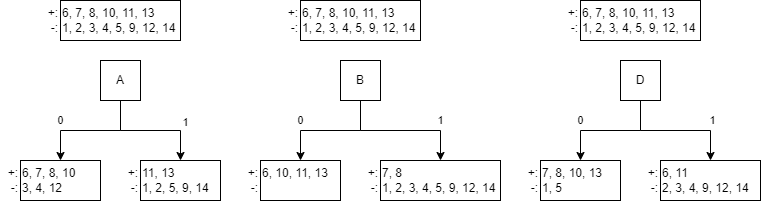
\includegraphics[width=0.75\textwidth]{Images/Question 4.png}
    \caption{Question 4 Decision Tree}
\end{figure}

\newpage
\problem{Information Gain}

\solution
The calculations for the infomation gained from $A,B,D$ are as follows
\begin{flalign*}
    Entropy(E)       & =-\frac{6}{14}\log_2\left(\frac{6}{14}\right)-\frac{8}{14}\log_2\left(\frac{8}{14}\right) & \\
                     & =0.985                                                                                    & \\
    Entropy(A_{E_0}) & =-\frac{4}{7}\log_2\left(\frac{4}{7}\right)-\frac{3}{7}\log_2\left(\frac{3}{7}\right)     & \\
                     & = 0.985                                                                                   & \\
    Entropy(A_{E_1}) & =-\frac{2}{7}\log_2\left(\frac{2}{7}\right)-\frac{5}{7}\log_2\left(\frac{5}{7}\right)     & \\
                     & = 0.863                                                                                   & \\
    Gain(E, A)       & = Entropy(E)-\frac{7}{14}Entropy(A_{E_0})-\frac{7}{14}Entropy(A_{E_1})                    & \\
                     & = 0.985-\frac{7}{14}(0.985)-\frac{7}{14}(0.863)                                           & \\
                     & = 0.061
\end{flalign*}


\noindent
\begin{flalign*}
    Entropy(B_{E_0}) & =-\frac{4}{4}\log_2\left(\frac{4}{4}\right)-\frac{0}{4}\log_2\left(\frac{0}{4}\right)     & \\
                     & = 0                                                                                       & \\
    Entropy(B_{E_1}) & =-\frac{2}{10}\log_2\left(\frac{2}{10}\right)-\frac{8}{10}\log_2\left(\frac{8}{10}\right) & \\
                     & = 0.722                                                                                   & \\
    Gain(E,B)        & = Entropy(E)-\frac{4}{14}Entropy(B_{E_0})-\frac{10}{14}Entropy(B_{E_1})                   & \\
                     & = 0.985-\frac{4}{14}(0)-\frac{10}{14}(0.722)                                              & \\
                     & = 1.469
\end{flalign*}

\noindent
\begin{flalign*}
    Entropy(D_{E_0}) & =-\frac{4}{6}\log_2\left(\frac{4}{6}\right)-\frac{2}{6}\log_2\left(\frac{2}{6}\right) & \\
                     & = 0.918                                                                               & \\
    Entropy(D_{E_1}) & =-\frac{2}{8}\log_2\left(\frac{2}{8}\right)-\frac{6}{8}\log_2\left(\frac{6}{8}\right) & \\
                     & = 0.811                                                                               & \\
    Gain(E, D)       & = Entropy(E)-\frac{6}{14}Entropy(D_{E_0})-\frac{8}{14}Entropy(D_{E_1})                & \\
                     & = 0.985-\frac{6}{14}(0.918)-\frac{8}{14}(0.811)                                       & \\
                     & = 0.128
\end{flalign*}

\noindent
Based on the calculated values for the information gains, we should test Attribute $B$ first since it has the highest information gain.

\problem Programming Information Gain

\solution The code is included in the submission folder as requested.

\newpage
\problem Decision Tree

\solution
\begin{figure}[!ht]
    \centering
    \begin{subfigure}{0.5\textwidth}
        \centering
        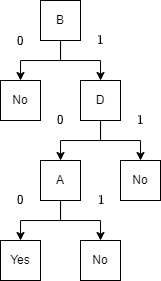
\includegraphics[height=256px]{Images/Question 7 Simplified.png}
        \caption{Simplified Decision Tree}
    \end{subfigure}%
    \begin{subfigure}{0.5\textwidth}
        \centering
        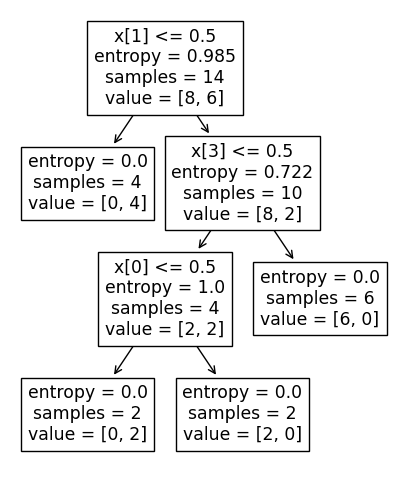
\includegraphics[height=256px]{Images/Question 7 Original.png}
        \caption{Original Decision Tree}
    \end{subfigure}
    \caption{Comparison of Decision Trees}
\end{figure}

\begin{figure}[!ht]
    \centering
    \begin{subfigure}{0.5\textwidth}
        \centering
        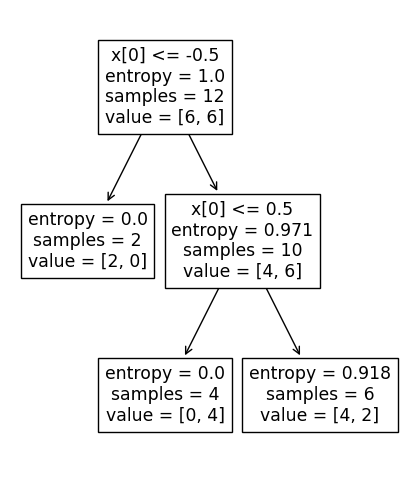
\includegraphics[height=256px]{Images/Question 7 Tree 1.png}
        \caption{Novel Tree 1}
    \end{subfigure}%
    \begin{subfigure}{0.5\textwidth}
        \centering
        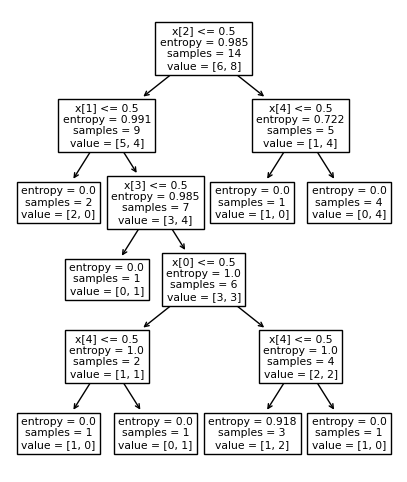
\includegraphics[height=256px]{Images/Question 7 Tree 2.png}
        \caption{Novel Tree 2}
    \end{subfigure}
    \caption{Novel Trees}
\end{figure}

\newpage
\problem Perceptron

\solution The code is included in the submission folder as requested.

\newpage
\problem Perceptron Drawing

\solution
\begin{figure}[!ht]
    \centering
    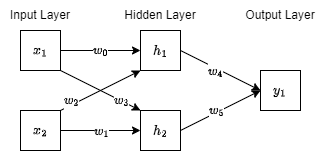
\includegraphics{Images/Question 9 Perceptron.png}
    \caption{XOR Perceptron}
\end{figure}

\begin{figure}[!ht]
    \centering
    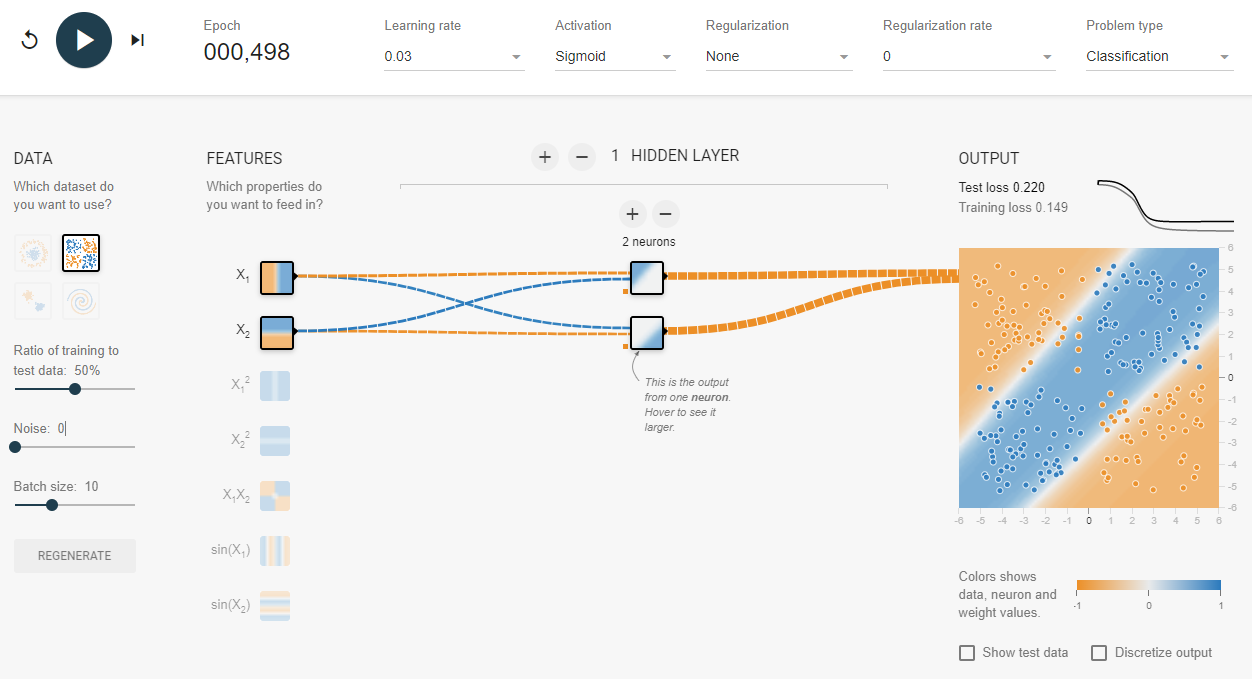
\includegraphics{Images/Question 9 Decision Boundary.png}
    \caption{XOR Decision Boundary}
\end{figure}

\end{document}
